\documentclass[11pt]{article}

% =================================================================
% PREAMBLE
% =================================================================
\usepackage[margin=1in]{geometry}
\usepackage{amsmath, amssymb, amsfonts}
\usepackage{graphicx}
\usepackage[colorlinks=true, urlcolor=blue, linkcolor=blue]{hyperref}
\usepackage{fancyhdr}
\usepackage{booktabs}   % For professional tables
\usepackage{multicol}   % For multi-column layout
\usepackage{enumitem}   % For customizing lists
\usepackage{tikz}       % For diagrams
\usepackage{xcolor}
\usepackage{adjustbox}  % For better figure scaling
\usepackage{array}      % For better table formatting
\usetikzlibrary{arrows.meta, positioning, decorations.pathreplacing}

% --- DOCUMENT INFORMATION ---
\title{Lecture 3: The Engine of Learning \\ From Loss Functions to Stochastic Gradient Descent}
\author{Building Intuition Step by Step}
\date{}

% --- HEADER/FOOTER ---
\pagestyle{fancy}
\fancyhf{}
\rhead{Lecture 3: The Engine of Learning}
\lhead{\thepage}

% --- MATH MACROS ---
\newcommand{\w}{\mathbf{w}}
\newcommand{\x}{\mathbf{x}}
\newcommand{\E}{\mathbb{E}}
\newcommand{\R}{\mathbb{R}}
\newcommand{\loss}{\mathcal{L}}

% --- HOMEWORK BOX ENVIRONMENT ---
\usepackage{tcolorbox}
\newtcolorbox{homeworkbox}[1][]{%
  colback=blue!5!white,
  colframe=blue!75!black,
  title={\textbf{Homework Problem}},
  fonttitle=\bfseries,
  #1
}

\begin{document}

\maketitle
\thispagestyle{empty}
\tableofcontents
\newpage

% =================================================================
\section{The Big Picture: What We're Trying to Do}
% =================================================================

Let's start with a concrete example to build our intuition. Imagine we're teaching a computer to recognize handwritten digits (0-9). We have:

\begin{itemize}
\item \textbf{Input}: A 28×28 pixel image (784 numbers between 0 and 1)
\item \textbf{Network}: A deep neural network $f(\x; \w)$ with millions of parameters $\w$
\item \textbf{Output}: 10 probabilities (one for each digit 0-9)
\item \textbf{Goal}: Make the network predict the correct digit
\end{itemize}

\begin{figure}[h!]
\centering
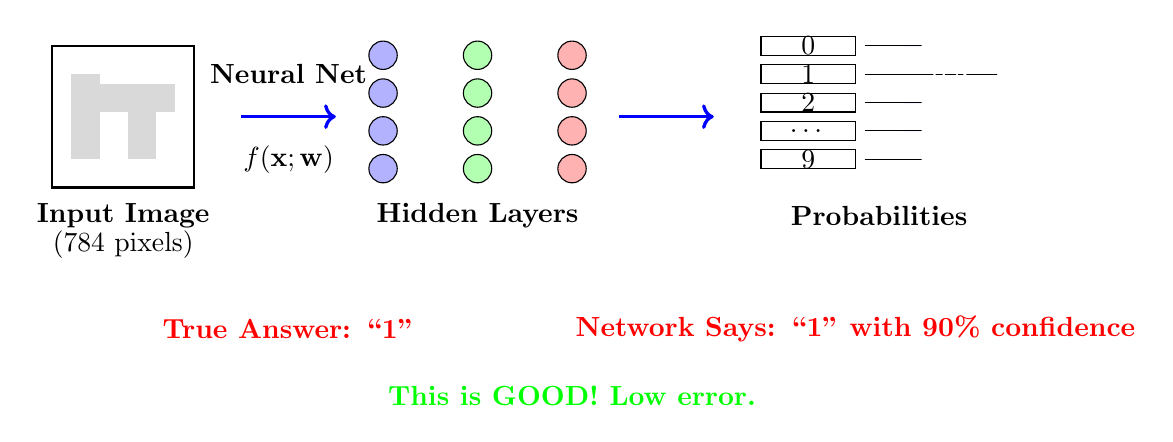
\begin{tikzpicture}[scale=1.2]
    % Input image representation
    \draw[thick] (0,0) rectangle (1.5,1.5);
    \fill[gray!30] (0.2,0.3) rectangle (0.5,1.2);
    \fill[gray!30] (0.5,0.8) rectangle (1.3,1.1);
    \fill[gray!30] (0.8,0.3) rectangle (1.1,0.8);
    \node at (0.75, -0.3) {\textbf{Input Image}};
    \node at (0.75, -0.6) {(784 pixels)};
    
    % Arrow
    \draw[->, very thick, blue] (2,0.75) -- (3,0.75);
    \node at (2.5, 1.2) {\textbf{Neural Net}};
    \node at (2.5, 0.3) {$f(\x; \w)$};
    
    % Network representation
    \foreach \y in {0.2,0.6,1.0,1.4} {
        \draw[fill=blue!30] (3.5, \y) circle (0.15);
        \draw[fill=green!30] (4.5, \y) circle (0.15);
        \draw[fill=red!30] (5.5, \y) circle (0.15);
    }
    \node at (4.5, -0.3) {\textbf{Hidden Layers}};
    
    % Arrow
    \draw[->, very thick, blue] (6,0.75) -- (7,0.75);
    
   % Output probabilities
    \foreach \i/\label in {0/0, 1/1, 2/2, 3/\ldots, 4/9} {
        \draw (7.5, {1.6-0.3*\i}) rectangle (8.5, {1.4-0.3*\i});
        \node at (8, {1.5-0.3*\i}) {\label};
        \draw[-] (8.6, {1.5-0.3*\i}) -- (9, {1.5-0.3*\i});
        \ifnum\i=1
            \draw[fill=red!50] (9, {1.5-0.3*\i}) rectangle (10, {1.5-0.3*\i});
            \node[white] at (9.5, {1.5-0.3*\i}) {0.9};
        \else
            \draw[fill=blue!30] (9, {1.5-0.3*\i}) rectangle (9.2, {1.5-0.3*\i});
        \fi
    }
    \node at (8.75, -0.3) {\textbf{Probabilities}};
    
    % True label
    \node[red] at (2.5, -1.5) {\textbf{True Answer: ``1"}};
    \node[red] at (8.5, -1.5) {\textbf{Network Says: ``1" with 90\% confidence}};
    \node[green] at (5.5, -2.2) {\textbf{This is GOOD! Low error.}};
\end{tikzpicture}
\caption{The learning setup: We want our network to correctly classify images. When it gets the right answer with high confidence, the error is low.}
\label{fig:learning_setup}
\end{figure}

The fundamental question is: \textbf{How do we adjust the millions of parameters $\w$ to make the network better at this task?}

This is where we need two key ingredients:
\begin{enumerate}
\item \textbf{A way to measure ``how wrong" we are} $\rightarrow$ Loss Function
\item \textbf{A systematic way to improve} $\rightarrow$ Optimization Algorithm
\end{enumerate}

% =================================================================
\section{Building the Loss Function: Measuring Our Mistakes}
% =================================================================

\subsection{The Intuitive Idea}
Think of the loss function as a ``mistake meter." It should:
\begin{itemize}
\item Give a \textbf{small number} when our network is performing well
\item Give a \textbf{large number} when our network is making big mistakes
\item Be \textbf{differentiable} so we can use calculus to improve it
\end{itemize}

\subsection{Building It Step by Step}

Let's construct a loss function for our digit classification example:

\textbf{Step 1: Single Example Loss}\\
For one training example $(x_i, y_i)$ where $y_i$ is the true digit (0-9):
\begin{equation}
\ell_i(\w) = \text{some measure of error between prediction and truth}
\end{equation}

\textbf{Step 2: Multiple Examples}\\
We have $N$ training examples, so our total loss is:
\begin{equation}
\boxed{L(\w) = \frac{1}{N} \sum_{i=1}^{N} \ell_i(\w)}
\end{equation}

\begin{homeworkbox}
\textbf{Problem 1: Deriving Cross-Entropy Loss from Maximum Likelihood}

\textbf{Context}: You are building a digit classifier. Your neural network outputs a probability distribution over the 10 possible digits (0-9). Given an input image $\x_i$, the network produces probabilities $p_1, p_2, \ldots, p_{10}$ where $\sum_{j=1}^{10} p_j = 1$.

\textbf{Question}: Derive the cross-entropy loss function starting from the principle of Maximum Likelihood Estimation (MLE).

\textbf{Part (a)}: Write down the likelihood of observing the true labels $y_1, y_2, \ldots, y_N$ given your model's predictions. Assume each prediction is independent.

\textbf{Part (b)}: Convert this to a log-likelihood and explain why we want to maximize it.

\textbf{Part (c)}: Show that maximizing the log-likelihood is equivalent to minimizing the cross-entropy loss:
$$\ell_i(\w) = -\log(p_{y_i})$$
where $p_{y_i}$ is the predicted probability for the true class $y_i$.

\textbf{Part (d)}: Explain intuitively why this loss function makes sense by considering what happens when:
\begin{itemize}
\item The model is very confident and correct ($p_{y_i} \approx 1$)
\item The model is very confident but wrong ($p_{y_i} \approx 0$)
\item The model is uncertain ($p_{y_i} \approx 0.1$ for 10-class problem)
\end{itemize}
\end{homeworkbox}

\textbf{Step 3: Cross-Entropy Loss Visualization}

\begin{figure}[h!]
\centering
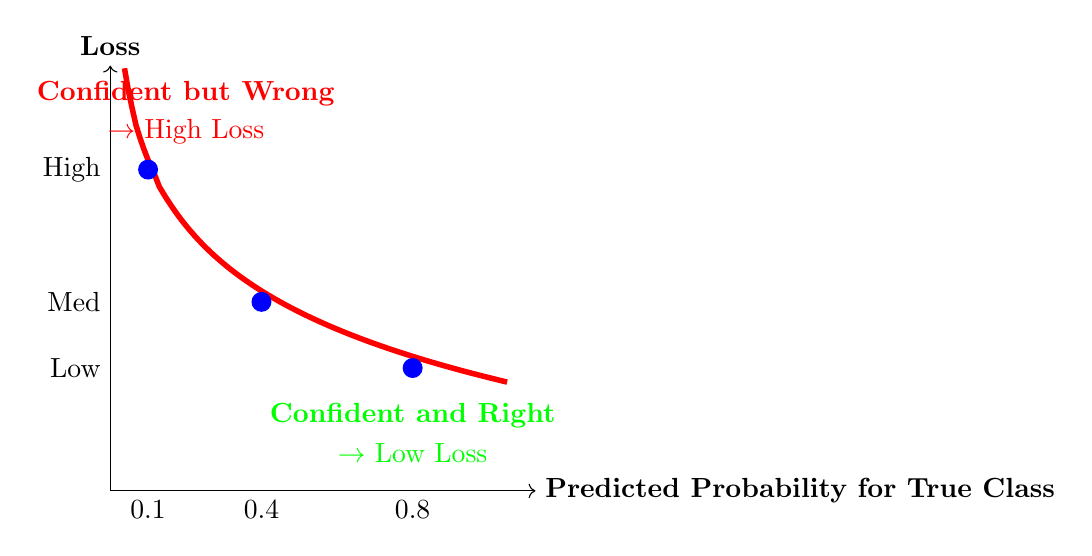
\begin{tikzpicture}[scale=1.2]
    % Graph of -log(p)
    \draw[->] (0,0) -- (4.5,0) node[right] {\textbf{Predicted Probability for True Class}};
    \draw[->] (0,0) -- (0,4.5) node[above] {\textbf{Loss}};
    
    % Draw the curve -log(p)
    \draw[thick, red, line width=2pt, domain=0.15:4.2, samples=100] 
          plot (\x, {-ln(\x/4) + 1.2});
    
    % Mark important points
    \fill[blue] (0.4, 3.4) circle (3pt);
    \fill[blue] (1.6, 2.0) circle (3pt);
    \fill[blue] (3.2, 1.3) circle (3pt);
    
    % Labels
    \node[below] at (0.4, 0) {0.1};
    \node[below] at (1.6, 0) {0.4};
    \node[below] at (3.2, 0) {0.8};
    \node[left] at (0, 3.4) {High};
    \node[left] at (0, 2.0) {Med};
    \node[left] at (0, 1.3) {Low};
    
    % Annotations
    \node[red] at (0.8, 4.2) {\textbf{Confident but Wrong}};
    \node[red] at (0.8, 3.8) {$\rightarrow$ High Loss};
    \node[green] at (3.2, 0.8) {\textbf{Confident and Right}};
    \node[green] at (3.2, 0.4) {$\rightarrow$ Low Loss};
\end{tikzpicture}
\caption{Cross-entropy loss: When the network is confident about the wrong answer, the loss is very high. When it's confident about the right answer, the loss is low.}
\label{fig:cross_entropy}
\end{figure}

% =================================================================
\section{The Optimization Challenge: Finding the Best Parameters}
% =================================================================

Now we have a clear objective: find the parameters $\w$ that minimize our loss function $L(\w)$:
\begin{equation}
\boxed{\w^* = \arg\min_{\w} L(\w) = \arg\min_{\w} \frac{1}{N} \sum_{i=1}^{N} \ell_i(\w)}
\end{equation}

But here's the challenge: In a modern neural network, $\w$ might have \textbf{billions} of parameters, and the loss function $L(\w)$ is incredibly complex and non-convex.

\subsection{The Hill-Climbing Analogy}
Imagine you're blindfolded on a hilly landscape (the loss surface) and want to find the lowest valley (minimum loss). You can:
\begin{itemize}
\item \textbf{Feel the slope} under your feet (compute the gradient)
\item \textbf{Take a step} in the direction that goes downhill (gradient descent)
\item \textbf{Repeat} until you reach a valley
\end{itemize}

\begin{figure}[h!]
\centering
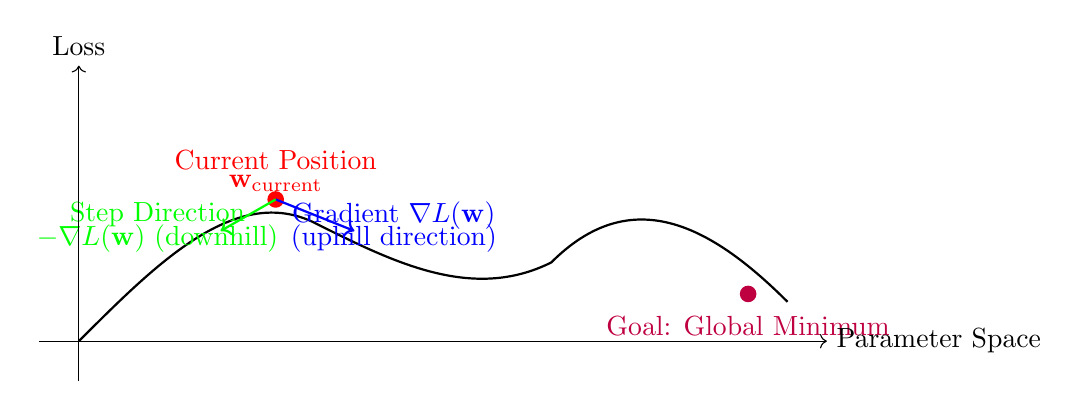
\begin{tikzpicture}[scale=1.0]
    % Draw a loss landscape
    \draw[thick] (0,0) .. controls (1,1) and (2,2) .. (3,1.5) .. controls (4,1) and (5,0.5) .. (6,1) .. controls (7,2) and (8,1.5) .. (9,0.5);
    
    % Current position
    \fill[red] (2.5, 1.8) circle (3pt);
    \node[red] at (2.5, 2.3) {Current Position};
    \node[red] at (2.5, 2.0) {$\w_{\text{current}}$};
    
    % Gradient arrow
    \draw[->, thick, blue] (2.5, 1.8) -- (3.5, 1.4);
    \node[blue] at (4, 1.6) {Gradient $\nabla L(\w)$};
    \node[blue] at (4, 1.3) {(uphill direction)};
    
    % Step direction
    \draw[->, thick, green] (2.5, 1.8) -- (1.8, 1.4);
    \node[green] at (1, 1.6) {Step Direction};
    \node[green] at (1, 1.3) {$-\nabla L(\w)$ (downhill)};
    
    % Global minimum
    \fill[purple] (8.5, 0.6) circle (3pt);
    \node[purple] at (8.5, 0.2) {Goal: Global Minimum};
    
    % Axes
    \draw[->] (0,-0.5) -- (0,3.5) node[above] {Loss};
    \draw[->] (-0.5,0) -- (9.5,0) node[right] {Parameter Space};
\end{tikzpicture}
\caption{The optimization landscape: We start at some position in parameter space and follow the negative gradient (downhill direction) to find lower loss.}
\label{fig:optimization_landscape}
\end{figure}

% =================================================================
\section{Gradient Descent: The Basic Algorithm}
% =================================================================

The mathematical formulation of our hill-climbing intuition is \textbf{Gradient Descent}:

\begin{equation}
\boxed{\w_{\text{new}} = \w_{\text{old}} - \alpha \nabla L(\w_{\text{old}})}
\end{equation}

Where:
\begin{itemize}
\item $\nabla L(\w)$ is the gradient (vector of partial derivatives)
\item $\alpha$ is the \textbf{learning rate} (step size)
\end{itemize}

\begin{homeworkbox}
\textbf{Problem 2: Gradient Descent vs. Closed-Form Solution for Linear Regression}

\textbf{Context}: You want to fit a line $y = w_1 x + w_2$ to the following data points: $(1, 3), (2, 5), (3, 7), (4, 9)$. You'll solve this problem both analytically and with gradient descent.

\textbf{Part (a): Analytical Solution}
\begin{enumerate}
\item Write the Mean Squared Error loss function $L(w_1, w_2)$
\item Set up the normal equations by setting $\nabla L = 0$
\item Solve for the optimal parameters $w_1^*, w_2^*$ analytically
\item What is the minimum loss value?
\end{enumerate}

\textbf{Part (b): Gradient Descent Solution}
\begin{enumerate}
\item Derive the partial derivatives $\frac{\partial L}{\partial w_1}$ and $\frac{\partial L}{\partial w_2}$
\item Starting from $w_1^{(0)} = 0, w_2^{(0)} = 0$ with learning rate $\alpha = 0.1$, perform 3 iterations of gradient descent
\item Show your calculations for each step
\item How close are you to the analytical solution after 3 steps?
\end{enumerate}

\textbf{Part (c): Comparison and Analysis}
\begin{enumerate}
\item Compare the computational complexity: How many operations does the analytical solution require vs. gradient descent?
\item When would you prefer gradient descent over the analytical solution?
\item What happens if you use a learning rate that's too large ($\alpha = 1.0$)?
\end{enumerate}

\textbf{Bonus}: Plot the loss function contours and show the gradient descent path.
\end{homeworkbox}

% =================================================================
\section{The Computational Bottleneck}
% =================================================================

Gradient descent works beautifully in theory, but there's a massive practical problem. To compute the true gradient, we need to sum over \textit{all} training examples:

\begin{equation}
\nabla L(\w) = \frac{1}{N} \sum_{i=1}^{N} \nabla \ell_i(\w)
\end{equation}

\textbf{The Scale Problem}:
\begin{itemize}
\item Modern datasets: $N =$ millions to billions of examples
\item Modern networks: $|\w| =$ millions to billions of parameters
\item Computing one gradient step requires looking at \textit{every single example}
\item This can take hours for just one step!
\item Training typically requires thousands of steps
\end{itemize}

\begin{figure}[h!]
\centering
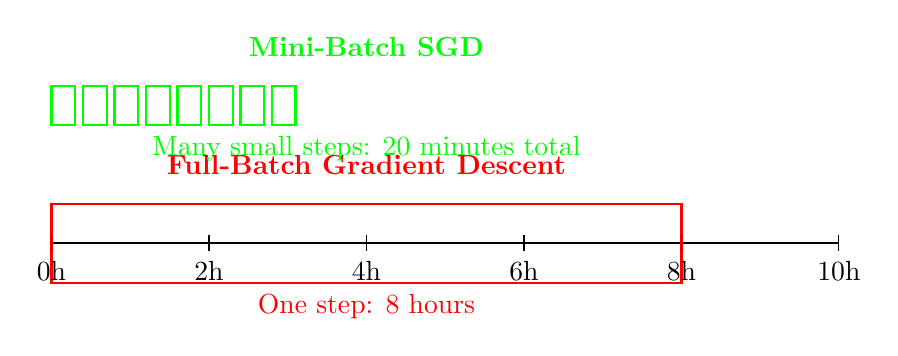
\begin{tikzpicture}[scale=1.0]
    % Timeline
    \draw[thick] (0,1) -- (10,1);
    
    % Full batch step
    \draw[red, thick] (0,0.5) rectangle (8,1.5);
    \node[red] at (4, 2) {\textbf{Full-Batch Gradient Descent}};
    \node[red] at (4, 0.2) {One step: 8 hours};
    
    % Mini-batch steps
    \foreach \x in {0, 0.4, 0.8, 1.2, 1.6, 2.0, 2.4, 2.8} {
        \draw[green, thick] (\x, 2.5) rectangle (\x+0.3, 3);
    }
    \node[green] at (4, 3.5) {\textbf{Mini-Batch SGD}};
    \node[green] at (4, 2.2) {Many small steps: 20 minutes total};
    
    % Time markers
    \foreach \x in {0,2,4,6,8,10} {
        \draw (\x, 0.9) -- (\x, 1.1);
        \node[below] at (\x, 0.9) {\x h};
    }
\end{tikzpicture}
\caption{The computational bottleneck: Full-batch gradient descent takes forever, while mini-batch SGD makes many quick progress steps in the same time.}
\label{fig:computational_bottleneck}
\end{figure}

% =================================================================
\section{Stochastic Gradient Descent: The Game-Changing Solution}
% =================================================================

The brilliant insight of Stochastic Gradient Descent (SGD) is simple: \textbf{We don't need the exact gradient—a good approximation is enough!}

\subsection{The Core Idea}
Instead of computing the expensive exact gradient:
\begin{equation}
\nabla L(\w) = \frac{1}{N} \sum_{i=1}^{N} \nabla \ell_i(\w) \quad \text{(expensive)}
\end{equation}

We approximate it using a small random \textbf{mini-batch}:
\begin{equation}
\nabla L_{\text{batch}}(\w) = \frac{1}{B} \sum_{i \in \text{batch}} \nabla \ell_i(\w) \quad \text{(cheap!)}
\end{equation}

Where $B \ll N$ (e.g., $B = 32$ while $N = 1,000,000$).

\subsection{Why Does This Possibly Work? A Simple Proof}
This seems reckless—how can a tiny sample represent the entire dataset? Let's prove that this approximation is \textbf{unbiased} with a simple argument.

\begin{figure}[h!]
\centering
\fbox{\begin{minipage}{0.9\textwidth}
\textbf{Intuitive Proof: Mini-batch Gradient is Unbiased}

\textbf{Setup:} 
\begin{itemize}
\item Full dataset: $N$ examples with individual losses $\ell_1(\w), \ell_2(\w), \ldots, \ell_N(\w)$
\item True gradient: $\nabla L(\w) = \frac{1}{N} \sum_{i=1}^{N} \nabla \ell_i(\w)$
\item Mini-batch: Randomly select $B$ examples from the $N$ examples
\end{itemize}

\textbf{Key Insight:} When we randomly sample, each example has an equal chance of being selected.

\textbf{Step 1:} For any specific example $i$, what's the probability it's in our mini-batch?
\begin{align}
P(\text{example } i \text{ is selected}) = \frac{B}{N}
\end{align}

\textbf{Step 2:} What's the expected contribution of example $i$ to our mini-batch gradient?
\begin{align}
\mathbb{E}[\text{contribution of example } i] &= P(\text{selected}) \times \frac{1}{B} \nabla \ell_i(\w) + P(\text{not selected}) \times 0 \\
&= \frac{B}{N} \times \frac{1}{B} \nabla \ell_i(\w) + \left(1-\frac{B}{N}\right) \times 0 \\
&= \frac{1}{N} \nabla \ell_i(\w)
\end{align}

\textbf{Step 3:} Expected value of the entire mini-batch gradient:
\begin{align}
\mathbb{E}[\nabla L_{\text{batch}}(\w)] &= \mathbb{E}\left[\sum_{i=1}^{N} \text{contribution of example } i\right] \\
&= \sum_{i=1}^{N} \mathbb{E}[\text{contribution of example } i] \\
&= \sum_{i=1}^{N} \frac{1}{N} \nabla \ell_i(\w) \\
&= \frac{1}{N} \sum_{i=1}^{N} \nabla \ell_i(\w) = \nabla L(\w)
\end{align}

\textbf{Conclusion:} $\boxed{\mathbb{E}[\nabla L_{\text{batch}}(\w)] = \nabla L(\w)}$ $\checkmark$
\end{minipage}}
\end{figure}

\textbf{Important Caveat - Sampling Without Replacement:}
In practice, we don't sample with replacement. We shuffle the dataset and partition it into mini-batches. This means:
\begin{itemize}
\item Each example appears exactly once per epoch
\item The mini-batch gradient is still unbiased \textit{on average across different epochs}
\item Within a single epoch, there's slight correlation between mini-batches, but this doesn't hurt performance
\item This approach is actually \textit{better} than sampling with replacement because it ensures we see all data
\end{itemize}

\textbf{In Plain English}: 
\begin{itemize}
\item Each example contributes to the mini-batch gradient with probability $\frac{B}{N}$
\item When it contributes, it gets weight $\frac{1}{B}$ in the mini-batch
\item On average, each example contributes exactly $\frac{1}{N}$ to the expected gradient
\item This is exactly the same weight it has in the true gradient!
\end{itemize}

\begin{figure}[h!]
\centering
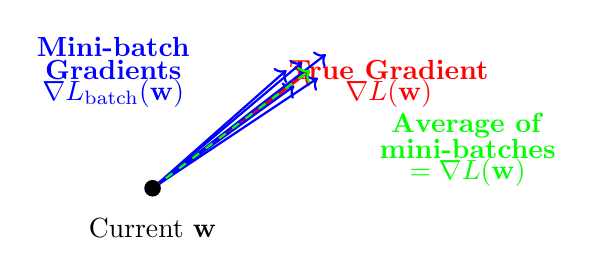
\begin{tikzpicture}[scale=1.0]
    % True gradient
    \draw[->, very thick, red] (2,2) -- (4,3.5);
    \node[red] at (5, 3.5) {\textbf{True Gradient}};
    \node[red] at (5, 3.2) {$\nabla L(\w)$};
    
    % Mini-batch gradients
    \draw[->, thick, blue] (2,2) -- (3.8,3.3);
    \draw[->, thick, blue] (2,2) -- (4.2,3.7);
    \draw[->, thick, blue] (2,2) -- (3.9,3.6);
    \draw[->, thick, blue] (2,2) -- (4.1,3.4);
    \draw[->, thick, blue] (2,2) -- (3.7,3.5);
    
    \node[blue] at (1.5, 3.8) {\textbf{Mini-batch}};
    \node[blue] at (1.5, 3.5) {\textbf{Gradients}};
    \node[blue] at (1.5, 3.2) {$\nabla L_{\text{batch}}(\w)$};
    
    % Average
    \draw[->, thick, green, dashed] (2,2) -- (4,3.5);
    \node[green] at (6, 2.8) {\textbf{Average of}};
    \node[green] at (6, 2.5) {\textbf{mini-batches}};
    \node[green] at (6, 2.2) {$= \nabla L(\w)$};
    
    % Starting point
    \fill[black] (2,2) circle (3pt);
    \node[black] at (2, 1.5) {Current $\w$};
\end{tikzpicture}
\caption{SGD intuition: Individual mini-batch gradients are noisy but unbiased. On average, they point in the right direction.}
\label{fig:sgd_intuition}
\end{figure}

\subsection{The SGD Algorithm}
\begin{equation}
\boxed{\w_{\text{new}} = \w_{\text{old}} - \alpha \cdot \frac{1}{B} \sum_{i \in \text{batch}} \nabla \ell_i(\w_{\text{old}})}
\end{equation}

\textbf{Practical Steps}:
\begin{enumerate}
\item \textbf{Shuffle} the training data
\item \textbf{Divide} into mini-batches of size $B$
\item For each mini-batch:
   \begin{enumerate}
   \item Compute gradients for the $B$ examples
   \item Average them
   \item Update parameters
   \end{enumerate}
\item \textbf{Repeat} for multiple epochs
\end{enumerate}



\subsection{The Two Zones of SGD: Geometric Intuition}
The noisy nature of SGD gives it a characteristic two-phase behavior:
\begin{description}
    \item[The ``Far-Out'' Zone:] When our model is very wrong (i.e., far from the optimal weights), almost any random sample we pick will tell us to move in roughly the same, correct direction. In this phase, SGD makes rapid, consistent progress, much like a speedboat heading toward a distant shore.
    \item[The ``Region of Confusion'':] As our model gets closer to the optimal weights, the situation changes. Now, different random samples might give conflicting directions. One sample might say ``go left,'' another ``go right.'' The algorithm starts to ``bounce around'' the minimum.
\end{description}
This noisy bouncing isn't necessarily a bad thing! Many researchers believe this stochasticity helps the model avoid getting stuck in poor local minima and can lead to solutions that \textbf{generalize better} to new, unseen data. It prevents the model from ``memorizing'' the training set too perfectly.

\begin{figure}[h!]
\centering
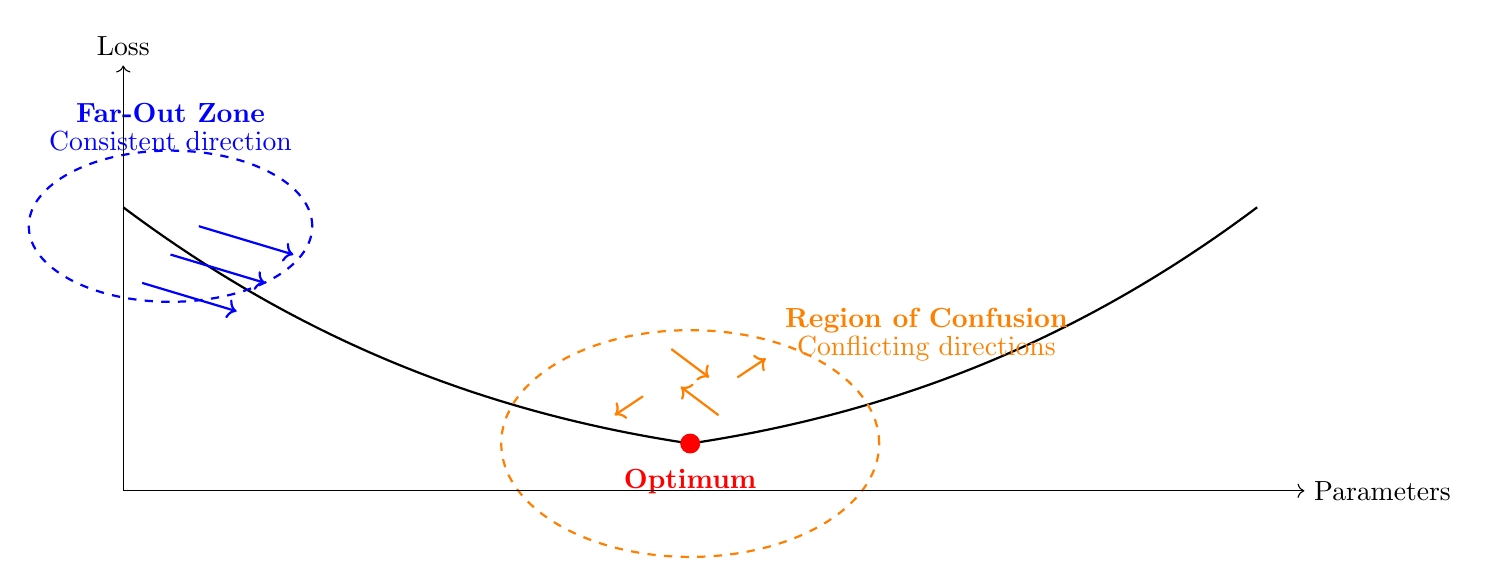
\begin{tikzpicture}[scale=1.2]
    % Draw loss landscape
    \draw[thick] (0,3) .. controls (2,1.5) and (4,0.8) .. (6,0.5) .. controls (8,0.8) and (10,1.5) .. (12,3);
    
    % Mark the minimum
    \fill[red] (6,0.5) circle (3pt);
    \node[red] at (6, 0.1) {\textbf{Optimum}};
    
    % Far-out zone
    \draw[blue, thick, dashed] (0.5, 2.8) ellipse (1.5 and 0.8);
    \node[blue] at (0.5, 4) {\textbf{Far-Out Zone}};
    \node[blue] at (0.5, 3.7) {Consistent direction};
    
    % Show consistent arrows in far-out zone
    \draw[->, blue, thick] (0.5, 2.5) -- (1.5, 2.2);
    \draw[->, blue, thick] (0.2, 2.2) -- (1.2, 1.9);
    \draw[->, blue, thick] (0.8, 2.8) -- (1.8, 2.5);
    
    % Region of confusion
    \draw[orange, thick, dashed] (6, 0.5) ellipse (2 and 1.2);
    \node[orange] at (8.5, 1.8) {\textbf{Region of Confusion}};
    \node[orange] at (8.5, 1.5) {Conflicting directions};
    
    % Show conflicting arrows in confusion zone
    \draw[->, orange, thick] (5.5, 1) -- (5.2, 0.8);
    \draw[->, orange, thick] (6.5, 1.2) -- (6.8, 1.4);
    \draw[->, orange, thick] (5.8, 1.5) -- (6.2, 1.2);
    \draw[->, orange, thick] (6.3, 0.8) -- (5.9, 1.1);
    
    % Axes
    \draw[->] (0,0) -- (0,4.5) node[above] {Loss};
    \draw[->] (0,0) -- (12.5,0) node[right] {Parameters};
\end{tikzpicture}
\caption{SGD's two zones: Far from the optimum, most samples point in the same helpful direction. Near the optimum, different samples give conflicting advice, causing beneficial ``bouncing.''}
\label{fig:sgd_zones}
\end{figure}

% =================================================================
\section{SGD's Secret Superpower: Escaping Bad Minima}
% =================================================================

The noise in SGD isn't just a necessary evil—it's often a \textbf{powerful feature}. Neural network loss landscapes are full of traps (local minima), and SGD's noise helps it escape these traps.

\subsection{The Local Minima Problem}
Consider this scenario: You're trying to find the deepest valley (global minimum), but there are many shallow puddles (local minima) that can trap you.

\begin{figure}[h!]
\centering
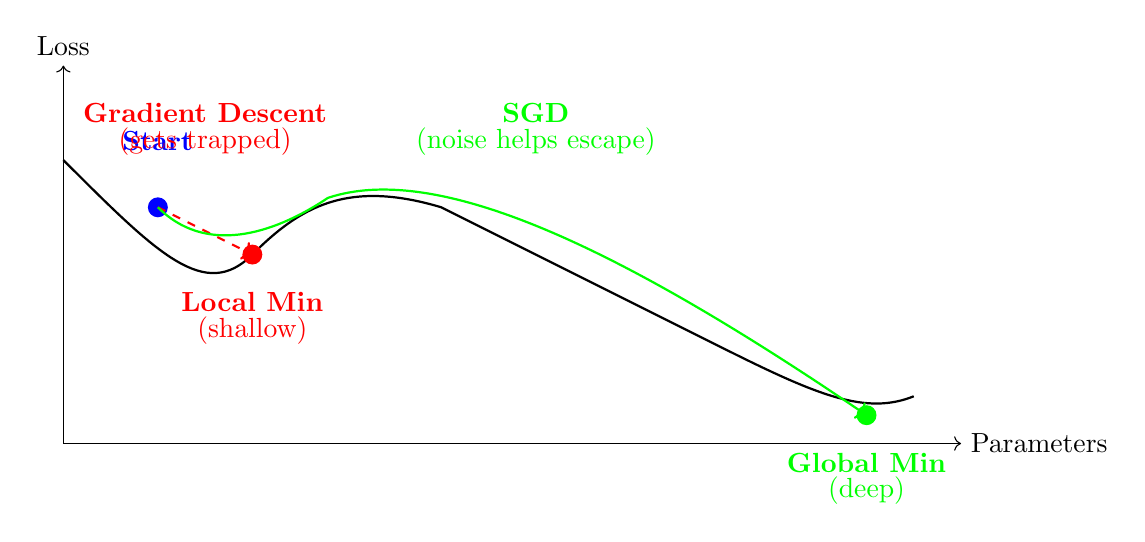
\begin{tikzpicture}[scale=1.2]
    % Loss landscape with multiple minima
    \draw[thick] (0,3) .. controls (1,2) and (1.5,1.5) .. (2,2) .. controls (2.5,2.5) and (3,2.8) .. (4,2.5) .. controls (5,2) and (6,1.5) .. (7,1) .. controls (8,0.5) and (8.5,0.3) .. (9,0.5);
    
    % Local minimum (shallow)
    \fill[red] (2,2) circle (3pt);
    \node[red] at (2, 1.5) {\textbf{Local Min}};
    \node[red] at (2, 1.2) {(shallow)};
    
    % Global minimum (deep)
    \fill[green] (8.5, 0.3) circle (3pt);
    \node[green] at (8.5, -0.2) {\textbf{Global Min}};
    \node[green] at (8.5, -0.5) {(deep)};
    
    % Starting point
    \fill[blue] (1, 2.5) circle (3pt);
    \node[blue] at (1, 3.2) {\textbf{Start}};
    
    % GD path (gets trapped)
    \draw[->, thick, red, dashed] (1, 2.5) -> (2, 2);
    \node[red] at (1.5, 3.5) {\textbf{Gradient Descent}};
    \node[red] at (1.5, 3.2) {(gets trapped)};
    
    % SGD path (escapes)
    \draw[->, thick, green] (1, 2.5) .. controls (1.5,2) and (2.2,2.2) .. (2.8,2.6) .. controls (4,3) and (6,2) .. (8.5, 0.3);
    \node[green] at (5, 3.5) {\textbf{SGD}};
    \node[green] at (5, 3.2) {(noise helps escape)};
    
    % Axes
    \draw[->] (0,0) -- (0,4) node[above] {Loss};
    \draw[->] (0,0) -- (9.5,0) node[right] {Parameters};
\end{tikzpicture}
\caption{SGD's superpower: The noise from mini-batches can kick the optimizer out of bad local minima, helping it find better solutions.}
\label{fig:escape_minima}
\end{figure}

\textbf{Why This Happens}:
\begin{itemize}
\item \textbf{Full-batch GD}: Deterministic path, gets stuck in first local minimum
\item \textbf{SGD}: Noisy updates can ``bounce" out of shallow minima
\item \textbf{Sharp vs. Flat Minima}: SGD tends to find flat, stable minima that generalize better
\end{itemize}


To visualize this, we can construct a 2D loss surface with a ``bad" (sharp, local) minimum and a ``good" (wider, global) minimum. We start both GD and SGD in a position where the steepest path leads directly to the bad minimum.

\begin{figure}[h!]
\centering
\includegraphics[width=0.9\textwidth]{figs/SGD.png}
\caption{A comparison of Gradient Descent (GD) and Mini-Batch SGD on a non-convex loss surface. Both optimizers start at the white star. The deterministic GD path (red) goes directly to the nearest (bad) local minimum and gets trapped. The noisy SGD path (cyan) initially explores the local minimum but its stochastic updates eventually ``kick" it out, allowing it to discover the deeper, more robust global minimum.}
\label{fig:sgd_vs_gd}
\end{figure}

% =================================================================
\section{Practical Considerations: Making SGD Work}
% =================================================================

\subsection{Choosing the Learning Rate $\alpha$}
The learning rate is crucial—it controls how big steps we take.

\begin{figure}[h!]
\centering
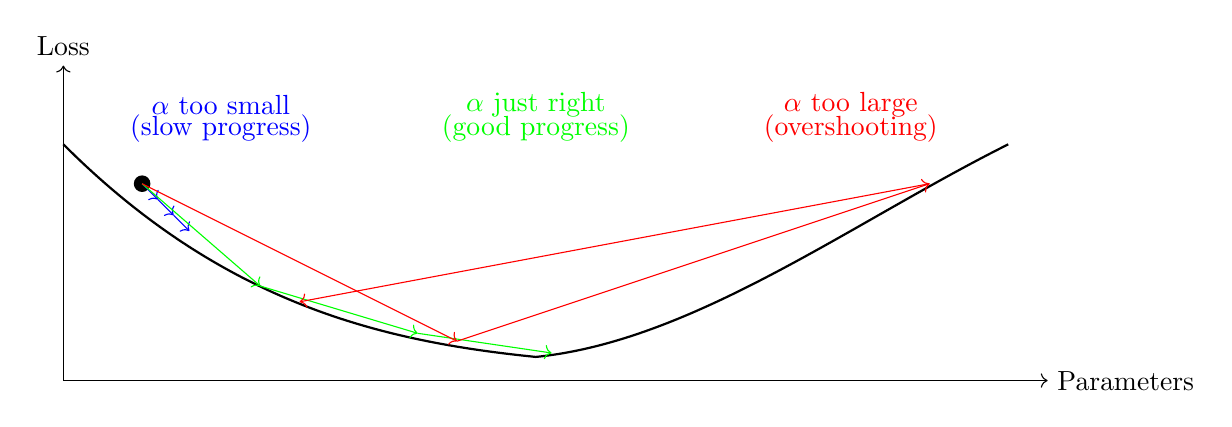
\begin{tikzpicture}[scale=1.0]
    % Loss curve
    \draw[thick] (0,3) .. controls (2,1) and (4,0.5) .. (6,0.3) .. controls (8,0.5) and (10,2) .. (12,3);
    
    % Starting point
    \fill[black] (1,2.5) circle (3pt);
    
    % Too small learning rate
    \draw[->, blue] (1,2.5) -- (1.2,2.3);
    \draw[->, blue] (1.2,2.3) -- (1.4,2.1);
    \draw[->, blue] (1.4,2.1) -- (1.6,1.9);
    \node[blue] at (2, 3.5) {$\alpha$ too small};
    \node[blue] at (2, 3.2) {(slow progress)};
    
    % Good learning rate
    \draw[->, green] (1,2.5) -- (2.5,1.2);
    \draw[->, green] (2.5,1.2) -- (4.5,0.6);
    \draw[->, green] (4.5,0.6) -- (6.2,0.35);
    \node[green] at (6, 3.5) {$\alpha$ just right};
    \node[green] at (6, 3.2) {(good progress)};
    
    % Too large learning rate
    \draw[->, red] (1,2.5) -- (5,0.5);
    \draw[->, red] (5,0.5) -- (11,2.5);
    \draw[->, red] (11,2.5) -- (3,1);
    \node[red] at (10, 3.5) {$\alpha$ too large};
    \node[red] at (10, 3.2) {(overshooting)};
    
    % Axes
    \draw[->] (0,0) -- (0,4) node[above] {Loss};
    \draw[->] (0,0) -- (12.5,0) node[right] {Parameters};
\end{tikzpicture}
\caption{Learning rate selection: Too small and progress is slow; too large and we overshoot the minimum.}
\label{fig:learning_rate}
\end{figure}

\textbf{Typical values}: $\alpha \in [0.001, 0.1]$\\
\textbf{Rule of thumb}: Start with $\alpha = 0.01$ and adjust based on training behavior.

\subsection{Choosing the Batch Size $B$}
Batch size is a crucial trade-off:

\begin{table}[h!]
\centering
\begin{tabular}{@{}lcc@{}}
\toprule
\textbf{Batch Size} & \textbf{Advantages} & \textbf{Disadvantages} \\
\midrule
Small (1-32) & High noise (good exploration) & Slow convergence \\
 & Better generalization & Inefficient on GPUs \\
\midrule
Medium (32-256) & Good balance & Moderate noise \\
 & Efficient on hardware & \\
\midrule
Large (512+) & Fast convergence & Less exploration \\
 & Very efficient & May overfit \\
\bottomrule
\end{tabular}
\caption{Batch size trade-offs}
\label{tab:batch_size}
\end{table}

\textbf{Sweet spot}: Usually $B \in [32, 128]$ for most applications.

% =================================================================
\section{Modern Improvements: Beyond Vanilla SGD}
% =================================================================

\subsection{SGD with Momentum}
Problem: SGD can oscillate in narrow valleys, slowing progress.\\
Solution: Add ``momentum" to smooth out the path.

\begin{align}
v_t &= \beta v_{t-1} + \nabla L(\w_t) \quad \text{(velocity update)} \\
\w_{t+1} &= \w_t - \alpha v_t \quad \text{(parameter update)}
\end{align}

Where $\beta \in [0.9, 0.99]$ is the momentum coefficient.

\textbf{Intuition}: Like a ball rolling downhill—it builds up speed in consistent directions and rolls through small bumps.

\begin{figure}[h!]
\centering
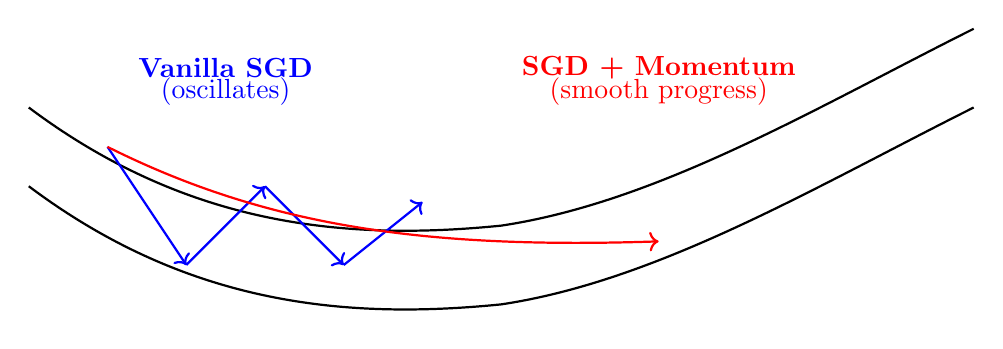
\begin{tikzpicture}[scale=1.0]
    % Valley landscape
    \draw[thick] (0,2) .. controls (2,0.5) and (4,0.3) .. (6,0.5) .. controls (8,0.8) and (10,2) .. (12,3);
    \draw[thick] (0,3) .. controls (2,1.5) and (4,1.3) .. (6,1.5) .. controls (8,1.8) and (10,3) .. (12,4);
    
    % SGD path (oscillating)
    \draw[->, blue, thick] (1,2.5) -- (2,1);
    \draw[->, blue, thick] (2,1) -- (3,2);
    \draw[->, blue, thick] (3,2) -- (4,1);
    \draw[->, blue, thick] (4,1) -- (5,1.8);
    \node[blue] at (2.5, 3.5) {\textbf{Vanilla SGD}};
    \node[blue] at (2.5, 3.2) {(oscillates)};
    
    % Momentum path (smooth)
    \draw[->, red, thick] (1,2.5) .. controls (3,1.5) and (5,1.2) .. (8,1.3);
    \node[red] at (8, 3.5) {\textbf{SGD + Momentum}};
    \node[red] at (8, 3.2) {(smooth progress)};
\end{tikzpicture}
\caption{Momentum helps SGD navigate narrow valleys more efficiently by accumulating velocity in consistent directions.}
\label{fig:momentum}
\end{figure}

\subsection{Adam: The Popular Choice}
Adam combines momentum with adaptive learning rates for each parameter.

\textbf{Key ideas}:
\begin{itemize}
\item \textbf{Momentum}: Accumulate past gradients
\item \textbf{Adaptive rates}: Scale learning rate for each parameter based on gradient history
\item \textbf{Bias correction}: Account for initialization bias
\end{itemize}

\textbf{When to use what}:
\begin{itemize}
\item \textbf{SGD + Momentum}: Simple, reliable, good for large models
\item \textbf{Adam}: Good default choice, works well out-of-the-box
\item \textbf{Learning rate scheduling}: Reduce $\alpha$ during training for fine-tuning
\end{itemize}

% =================================================================
\section{Putting It All Together: The Training Loop}
% =================================================================

Here's the complete algorithm that powers modern deep learning:

\begin{figure}[h!]
\centering
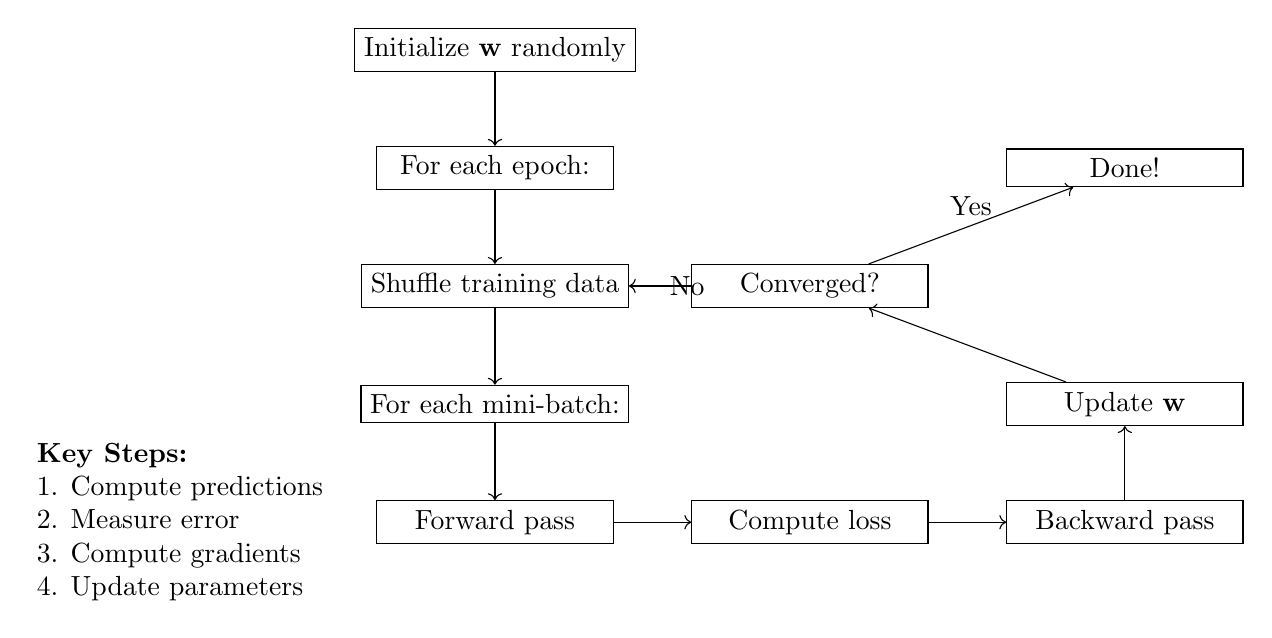
\begin{tikzpicture}[scale=1.0]
    % Flowchart boxes
    \node[draw, rectangle, minimum width=3cm] (start) at (0,8) {Initialize $\w$ randomly};
    \node[draw, rectangle, minimum width=3cm] (epoch) at (0,6.5) {For each epoch:};
    \node[draw, rectangle, minimum width=3cm] (shuffle) at (0,5) {Shuffle training data};
    \node[draw, rectangle, minimum width=3cm] (batch) at (0,3.5) {For each mini-batch:};
    \node[draw, rectangle, minimum width=3cm] (forward) at (0,2) {Forward pass};
    \node[draw, rectangle, minimum width=3cm] (loss) at (4,2) {Compute loss};
    \node[draw, rectangle, minimum width=3cm] (backward) at (8,2) {Backward pass};
    \node[draw, rectangle, minimum width=3cm] (update) at (8,3.5) {Update $\w$};
    \node[draw, rectangle, minimum width=3cm] (check) at (4,5) {Converged?};
    \node[draw, rectangle, minimum width=3cm] (done) at (8,6.5) {Done!};
    
    % Arrows
    \draw[->] (start) -- (epoch);
    \draw[->] (epoch) -- (shuffle);
    \draw[->] (shuffle) -- (batch);
    \draw[->] (batch) -- (forward);
    \draw[->] (forward) -- (loss);
    \draw[->] (loss) -- (backward);
    \draw[->] (backward) -- (update);
    \draw[->] (update) -- (check);
    \draw[->] (check) -- node[right] {No} (shuffle);
    \draw[->] (check) -- node[above] {Yes} (done);
    
    % Side annotations
    \node[align=left] at (-4, 2) {\textbf{Key Steps:}\\1. Compute predictions\\2. Measure error\\3. Compute gradients\\4. Update parameters};
\end{tikzpicture}
\caption{The complete training loop: This is the algorithm that trains neural networks to recognize images, translate languages, and more.}
\label{fig:training_loop}
\end{figure}

\newpage
% =================================================================
\section{What's Next: Computing Those Gradients}
% =================================================================

We've now seen the big picture of how neural networks learn. But there's one crucial piece missing:

\begin{center}
\Large\textbf{How do we actually compute $\nabla \ell_i(\w)$ for a deep network?}
\end{center}

A modern neural network might have billions of parameters, and the loss function is a deeply nested composition of functions. Computing these gradients by hand is impossible, and doing it naively on a computer would be incredibly slow.

This is where our next topic comes in: \textbf{Backpropagation}—the elegant algorithm that uses the chain rule of calculus to efficiently compute all gradients in one backward pass through the network.

\textbf{Coming up next}:
\begin{itemize}
\item \textbf{The Chain Rule}: How gradients flow backward through compositions
\item \textbf{Computational Graphs}: A visual way to understand complex functions
\item \textbf{Backpropagation}: The algorithm that made modern deep learning possible
\item \textbf{Implementation}: Writing our first neural network in code
\end{itemize}

Stay tuned—we're about to unlock the computational engine that powers all of modern AI!

\end{document}